%-----------------------------------------------------------------------
% Beginning of chapter.tex
%-----------------------------------------------------------------------
%
%  This is a sample file for use with AMS-LaTeX.  It provides an example
%  of how to set up a file for a book to be typeset with AMS-LaTeX.
%
%  This is the driver file.  Separate chapters should be included at
%  the end of this file.
%
%  ***** DO NOT USE THIS FILE AS A STARTER FOR YOUR BOOK. *****
%  Follow the guidelines in the file chapter.template.
%
%%%%%%%%%%%%%%%%%%%%%%%%%%%%%%%%%%%%%%%%%%%%%%%%%%%%%%%%%%%%%%%%%%%%%%%%

\documentclass[11pt,a4paper]{memoir}
\chapterstyle{demo}
\epigraphfontsize{\small\itshape}
\setlength\epigraphwidth{8cm}
\setlength\epigraphrule{0pt}
\epigraphfontsize{\small\itshape}
%\includeonly{preface,chap1,biblio}

%\numberwithin{section}{chapter}
%\numberwithin{equation}{chapter}

% Include macros here
%=================================================
% Packages
%=================================================

%\usepackage{fixltx2e}
\usepackage[usenames,dvipsnames]{xcolor}
%\usepackage{fancyhdr}
\usepackage{amsmath,amsfonts,amsbsy,amsgen,amscd,mathrsfs,amssymb,amscd}
\usepackage{amsthm}
\usepackage{bm}
\usepackage{url}
\usepackage[UKenglish]{babel}
\usepackage{eurosym}
\usepackage{tikz}
\usepackage{caption}
\usetikzlibrary{matrix,arrows,shapes,calc,3d}
\usepackage{tikz-3dplot}
\tdplotsetmaincoords{60}{110}
\pgfmathsetmacro{\rvec}{.8}
\pgfmathsetmacro{\thetavec}{30}
\pgfmathsetmacro{\phivec}{60}

\tikzset{mynode/.style = {
    % The shape
    circle,
    % The size
    minimum size=2pt,
    % The color
    draw=black, fill=black}
}
\tikzset{vertex/.style={shape=circle, % style for a vertex
                        minimum size=3pt,
                        fill=gray,
                        inner sep = 0pt}}  

% \usepackage{3dplot}
% \tdplotsetmaincoords{60}{110}
%\usepackage{subfig}
\usepackage{microtype}
\usepackage{enumitem}
\usepackage{listings}
\definecolor{darkblue}{rgb}{0,0,.75}

\usepackage[many]{tcolorbox}
\tcbuselibrary{listings}

\definecolor{light-gray}{rgb}{0.96,0.96,0.96}
\definecolor{kwgreen}{rgb}{0,0.5,0}
\definecolor{cogreen}{rgb}{0.25,0.5,0.5}
\definecolor{mygreen}{rgb}{0,0.5,0.125}
\definecolor{equalsign}{rgb}{0.66,0.13,1}
\definecolor{darkred}{rgb}{0.75,0.16,0.37}

\lstloadlanguages{Python} %use listings with Python
%\lstset{literate={==}{{\color{equalsign}==}} {\*}{{\color{equalsign}\*}}}
%\lstnewenvironment{PseudoCode}[1][]
% the space reserved between for the ``In'' numbers and the code
\newlength\inwd
\setlength\inwd{1.7cm}

\newcounter{ipythcntr}

\newtcblisting{ipythonnb}[1][\theipythcntr]{
  enlarge left by=\inwd,
  width=\linewidth-\inwd,
  enhanced,
  boxrule=0.4pt,
  boxsep=0pt,
  left=2pt,
  top=0pt,
  colback=light-gray,
  listing only,
  top=0pt,
  bottom=0pt,
  arc=1pt,
  overlay={
    \node[
      anchor=north east,
      text width=\inwd,
      font=\footnotesize\ttfamily\color{blue!50!black},
      inner ysep=2.5mm,
      inner xsep=0pt,
      outer sep=0pt
      ] 
      at (frame.north west)
      {\stepcounter{ipythcntr}In [#1]:};
  }
  listing style=Python,
  listing options={
    basicstyle=\scriptsize\ttfamily\color{black},
    language=Python,
    escapechar=£,
    showstringspaces=false,
    commentstyle=\color{cogreen},
    keywordstyle=\bfseries\color{kwgreen},
    stringstyle=\color{darkred},
    numberstyle=\color{kwgreen},
    identifierstyle=\color{black},
    %emph={from,import,as},          % Custom highlighting
    otherkeywords={0,1,2,3,4,5,6,7,8,9,\*,==,<=,>=,+,-,\%},
    emph={*,==,<=,>=,+,-,\%},    
    emphstyle=\color{equalsign},
    extendedchars=true,
  },
}

\newtcblisting{ipythonnbout}[1][\theipythcntr]{
  enlarge left by=\inwd,
  width=\linewidth-\inwd,
  enhanced,
  boxrule=0pt,
  boxsep=0pt,
  left=2pt,
  top=0pt,
  colback=white,
  listing only,
  top=0pt,
  bottom=0pt,
  frame hidden,
  overlay={
    \node[
      anchor=north east,
      text width=\inwd,
      font=\footnotesize\ttfamily\color{red},
      inner ysep=2.5mm,
      inner xsep=0pt,
      outer sep=0pt
      ] 
      at (frame.north west)
      {\stepcounter{ipythcntr}Out [#1]:};
  }
  listing style=Python,
  listing options={
    basicstyle=\scriptsize\ttfamily\color{black},
    language=Python,
    escapechar=£,
    showstringspaces=false,
    commentstyle=\color{cogreen},
    keywordstyle=\bfseries\color{kwgreen},
    stringstyle=\color{darkred},
    numberstyle=\color{kwgreen},
    identifierstyle=\color{black},
    %emph={from,import,as},          % Custom highlighting
%    otherkeywords={as,0,1,2,3,4,5,6,7,8,9,\*,==,<=,>=,+,-},
%    emph={*,==,<=,>=,+,-},    
%    emphstyle=\color{equalsign},
    extendedchars=true,
    %literate={#}{{\#}},
  },
}

\newtcblisting{ipythonnboutno}{
  enlarge left by=\inwd,
  width=\linewidth-\inwd,
  enhanced,
  boxrule=0pt,
  boxsep=0pt,
  left=2pt,
  top=0pt,
  colback=white,
  listing only,
  top=0pt,
  bottom=0pt,
  frame hidden,
  overlay={
    \node[
      anchor=north east,
      text width=\inwd,
      font=\footnotesize\ttfamily\color{red},
      inner ysep=2.5mm,
      inner xsep=0pt,
      outer sep=0pt
      ] 
      at (frame.north west)
      {};
  }
  listing style=Python,
  listing options={
    basicstyle=\scriptsize\ttfamily\color{black},
    language=Python,
    escapechar=£,
    showstringspaces=false,
    commentstyle=\color{cogreen},
    %keywordstyle=\bfseries\color{kwgreen},
    stringstyle=\color{darkred},
    numberstyle=\color{kwgreen},
    identifierstyle=\color{black},
    %emph={from,import,as},          % Custom highlighting
    %otherkeywords={as,0,1,2,3,4,5,6,7,8,9,\[,\]},
    %emph={[,]},    
    %emphstyle=\color{black},
    extendedchars=true,
    %literate={#}{{\#}},
  },
}


%{\lstset{language=Matlab,basicstyle=\small, keywordstyle=\color{darkblue},numbers=none,xleftmargin=.04\textwidth,mathescape,frame=single,#1}}
%{}
%\usepackage[]{algorithm2e}
%\usepackage{mcode}
\usepackage{multicol}

%\usepackage[draft]{changes}
%\definechangesauthor[color=blue]{ml}
%\definechangesauthor[color=red]{da}
% \usepackage{trackchanges}
% \addeditor{ml}
% \addeditor{da}

\definecolor{dark-gray}{gray}{0.3}
\definecolor{dkgray}{rgb}{.4,.4,.4}
\definecolor{dkblue}{rgb}{0,0,.5}
\definecolor{medblue}{rgb}{0,0,.75}
\definecolor{rust}{rgb}{0.5,0.1,0.1}

\usepackage[colorlinks=true]{hyperref}
\hypersetup{urlcolor=Blue}
\hypersetup{citecolor=Black}
\hypersetup{linkcolor=dark-gray}

%\usepackage{setspace}
\usepackage{graphicx}
%\usepackage{multicol}
\usepackage{booktabs,longtable,tabu} % Nice tables
\setlength{\tabulinesep}{1pt}
\usepackage{multirow} % More control over tables
\usepackage{float}
\usepackage[T1]{fontenc}
%\usepackage{quotchap}

% Fonts
\usepackage{times}
%\usepackage{fourier}
%\usepackage[no-math]{fontspec}
%\setmainfont{optima}
%\usepackage{charter}
\usepackage{bm} % boldmath must be called after the package

%=================================================
% Paths
%=================================================

\graphicspath{{figures/}}

%=================================================
% Formatting
%=================================================

%\sloppy % Helps with margin justification

%%% Further font changes
\newcommand{\lang}{\textit}
\newcommand{\titl}{\textsl}
\newcommand{\term}{\emph}

%%% Equation numbering
\numberwithin{equation}{section} 

%%% Typesetting
\providecommand{\mathbold}[1]{\bm{#1}}  % Must be after 'fourier'
                                % package loads
%%% Annotations
\newcommand{\notate}[1]{\textcolor{red}{\textbf{[#1]}}}

%=================================================
% Theorem environment
%=================================================

\newtheorem{bigthm}{Theorem}
\renewcommand{\thebigthm}{\Roman{bigthm}}

\newtheorem{theorem}{Theorem}[section]
\newtheorem{lemma}[theorem]{Lemma}
\newtheorem{sublemma}[theorem]{Sublemma}
\newtheorem{proposition}[theorem]{Proposition}
\newtheorem{fact}[theorem]{Fact}
\newtheorem{result}[theorem]{Result}
\newtheorem{conjecture}[theorem]{Conjecture}
\newtheorem{corollary}[theorem]{Corollary}

\newtheorem{problem}[theorem]{Problem}
\newtheorem{solution}[theorem]{Solution}

\theoremstyle{definition}

\newtheorem{definition}[theorem]{Definition}
\newtheorem{example}[theorem]{Example}
\newtheorem{remark}[theorem]{Remark}

\newenvironment{mainthm}{\par\textsc{Main theorem.}\it}{\par}
\renewcommand{\thebigthm}{\Alph{bigthm}}

%=================================================
% Symbols
%=================================================

%%% Old symbols with new names
\newcommand{\oldphi}{\phi}
\renewcommand{\phi}{\varphi}

\newcommand{\eps}{\varepsilon}
\newcommand{\e}{\varepsilon}

%\newcommand{\oldmid}{\mid}
\renewcommand{\mid}{\mathrel{\mathop{:}}} 

%%% New symbols
\newcommand{\defby}{\overset{\mathrm{\scriptscriptstyle{def}}}{=}}
\newcommand{\half}{\tfrac{1}{2}}
\newcommand{\third}{\tfrac{1}{3}}

\newcommand{\sumnl}{\sum\nolimits}

\newcommand{\defeq}{\ensuremath{\mathrel{\mathop{:}}=}} % Definition-equals
\newcommand{\eqdef}{\ensuremath{=\mathrel{\mathop{:}}}} % Equals-definition

%%% Constants
\newcommand{\cnst}[1]{\mathrm{#1}} 
\newcommand{\econst}{\mathrm{e}}
\newcommand{\iunit}{\mathrm{i}}

\newcommand{\onevct}{\mathbf{e}} % All ones vector
\newcommand{\zerovct}{\vct{0}} % Zero vector

\newcommand{\Id}{\mathbf{I}}
\newcommand{\onemtx}{\bm{1}}
\newcommand{\zeromtx}{\bm{0}}

%%% Sets
\newcommand{\coll}[1]{\mathscr{#1}}
\newcommand{\sphere}[1]{S^{#1}}
\newcommand{\ball}[1]{B^{#1}}
\newcommand{\Grass}[2]{\mathbb{G}(#1,#2)}
\providecommand{\mathbbm}{\mathbb} % In case we don't load bbm
\newcommand{\Rplus}{\mathbbm{R}_{+}}
\newcommand{\R}{\mathbbm{R}}
\newcommand{\C}{\mathbbm{C}}
\newcommand{\N}{\mathbbm{N}}
\newcommand{\FF}{\mathbbm{F}}
\newcommand{\struct}{\mathcal{S}}

% Group theory
\newcommand{\stab}{\mathrm{stab}}

% Algebra
\newcommand{\End}{\mathrm{End}}
\newcommand{\Hom}{\mathrm{Hom}}
\newcommand{\Mult}{\mathrm{Mult}}

% Set operations
\newcommand{\polar}{\circ}
\newcommand{\closure}{\overline}
\newcommand{\prtensor}{\,\hat{\otimes}\,}

%%% Real and complex analysis
\newcommand{\abs}[1]{\left\vert {#1} \right\vert}
\newcommand{\abssq}[1]{{\abs{#1}}^2}

\newcommand{\sgn}[1]{\operatorname{sgn}{#1}}
\newcommand{\real}{\operatorname{Re}}
\newcommand{\imag}{\operatorname{Im}}
\newcommand{\pos}{\operatorname{Pos}}
\newcommand{\shrink}{\operatorname{Shrink}}

\newcommand{\diff}[1]{\mathrm{d}{#1}}
\newcommand{\idiff}[1]{\, \diff{#1}}

\newcommand{\gradd}{\mathrm{grad }} % Conflicts w/SIAM styles?
\newcommand{\divv}{\mathrm{div }}
\newcommand{\subdiff}{\partial}

%%% Optimization

\newcommand{\minimize}{\text{minimize}\quad}
\newcommand{\maximize}{\text{maximize}\quad}
\newcommand{\subjto}{\quad\text{subject to}\quad}
\newcommand{\find}{\text{find}\quad}
\newcommand{\suchthat}{\quad\text{such that}\quad}

\newcommand{\argmin}{\operatorname*{arg\; min}}
\newcommand{\argmax}{\operatorname*{arg\; max}}
\newcommand{\dom}{\mathrm{dom} }

%%% Probability & measure

\newcommand{\Prob}{\mathbbm{P}}
\newcommand{\Probe}[1]{\Prob\left({#1}\right)}
\newcommand{\Expect}{\operatorname{\mathbb{E}}}

\newcommand{\St}{\operatorname{St}}

%\newcommand{\normal}{\textsc{Normal}}
\newcommand{\normal}{N}
\newcommand{\uniform}{\textsc{Uniform}}
\newcommand{\erf}{\operatorname{erf}}

\DeclareMathOperator{\rvol}{rvol}
\DeclareMathOperator{\Var}{Var}
\DeclareMathOperator{\Gl}{Gl}
\newcommand{\diag}{\operatorname{diag}}

%%% Vector and matrix operators
\newcommand{\vct}[1]{\mathbold{#1}}
\newcommand{\mtx}[1]{\mathbold{#1}}
\newcommand{\Eye}{\mathbf{I}}

\newcommand{\transp}[1]{#1^{T}}
\newcommand{\trans}{\top}
\newcommand{\adj}{*}
\newcommand{\psinv}{\dagger}

\newcommand{\lspan}[1]{\operatorname{span}{#1}}

\newcommand{\range}{\operatorname{range}}
\newcommand{\colspan}{\operatorname{colspan}}

%\newcommand{\rank}{\operatorname{rank}}
\newcommand{\nullity}{\operatorname{null}}
%\newcommand{\ker}{\operatorname{ker}}
\newcommand{\im}{\operatorname{im}}
%\newcommand{\span}{\operatorname{span}}

%\newcommand{\diag}{\operatorname{diag}}
\newcommand{\trace}{\operatorname{tr}}

\newcommand{\supp}[1]{\operatorname{supp}(#1)}
\newcommand{\sign}[1]{\operatorname{sign}(#1)}

\newcommand{\smax}{\sigma_{\max}}
\newcommand{\smin}{\sigma_{\min}}

\newcommand{\nnz}{\operatorname{nnz}}
\renewcommand{\vec}{\operatorname{vec}}

\newcommand{\Proj}{\ensuremath{\mtx{\Pi}}} % Projection operator

%%% Semidefinite orders
\newcommand{\psdle}{\preccurlyeq}
\newcommand{\psdge}{\succcurlyeq}

\newcommand{\psdlt}{\prec}
\newcommand{\psdgt}{\succ}

%%% Mensuration: inner products and norms

% TeX does not like either \newcommand or \renewcommand for these
% two macros.  There is probably a good reason not to use them via
% \def, but I don't know it.  
%\newcommand{\<}{\langle} 
%\newcommand{\>}{\rangle}
\newcommand{\ip}[2]{\langle {#1}, {#2} \rangle}
% --deleted the \left and \right-- Dennis
% \newcommand{\ip}[2]{\left\langle {#1},\ {#2} \right\rangle}
\newcommand{\absip}[2]{\abs{\ip{#1}{#2}}}
\newcommand{\abssqip}[2]{\abssq{\ip{#1}{#2}}}
\newcommand{\tworealip}[2]{2 \, \real{\ip{#1}{#2}}}

%\newcommand{\norm}[1]{\left\Vert {#1} \right\Vert}
\newcommand{\norm}[1]{\Vert {#1}\Vert}
\newcommand{\normsq}[1]{\norm{#1}^2}

\newcommand{\lone}[1]{\norm{#1}_{\ell_1}}
\newcommand{\smlone}[1]{\|#1\|_{\ell_1}}
\newcommand{\linf}[1]{\norm{#1}_{\ell_\infty}}
\newcommand{\sone}[1]{\norm{#1}_{S_1}}
\newcommand{\snorm}[1]{\sone{#1}}
\newcommand{\wnnorm}[1]{\norm{#1}_{*,\vct{w}}}
\newcommand{\wnnormd}[1]{\norm{#1}^*_{\vct{w}}}
\DeclareMathOperator{\dist}{dist}

% Fixed-size inner products and norms are useful sometimes
\newcommand{\smip}[2]{\bigl\langle {#1}, \ {#2} \bigr\rangle}
\newcommand{\smabsip}[2]{\bigl\vert \smip{#1}{#2} \bigr\vert}
\newcommand{\smnorm}[2]{{\bigl\Vert {#2} \bigr\Vert}_{#1}}

% Specific norms that are used frequently
\newcommand{\enormdangle}{{\ell_2}}
\newcommand{\enorm}[1]{\norm{#1}}
\newcommand{\enormsm}[1]{\enorm{\smash{#1}}}

\newcommand{\enormsq}[1]{\enorm{#1}^2}

\newcommand{\fnorm}[1]{\norm{#1}_{\mathrm{F}}}
\newcommand{\fnormsq}[1]{\fnorm{#1}^2}

\newcommand{\pnorm}[2]{\norm{#2}_{#1}}
%\newcommand{\snorm}[1]{\norm{#1}_*}

\newcommand{\triplenorm}[1]{\left\vert\!\left\vert\!\left\vert {#1} \right\vert\!\right\vert\!\right\vert} 

\newcommand{\flag}[2]{{#1 \brack #2}}

% Special cones
\newcommand{\Feas}{\mathcal{F}}
\newcommand{\Desc}{\mathcal{D}}

\newcommand{\sdim}{\delta}
\newcommand{\sdimw}{\delta^*}
% \newcommand{\sdimw}{\tilde{\delta}}
\newcommand{\ddt}[1]{\dot{#1}}
\DeclareMathOperator{\Circ}{Circ}

%%% Differential geometry
\newcommand{\Cinf}{C^{\infty}}
\newcommand{\Tensf}{\mathcal{T}}
\newcommand{\Vbundle}{\mathcal{X}}
\newcommand{\Christ}[3]{\Gamma_{{#1}{#2}}^{#3}}

% Stuff to be sorted in somewhere
\DeclareMathOperator{\Lip}{Lip}

\newcommand{\IR}{\mathbbm{R}}
\newcommand{\veps}{\varepsilon}
\newcommand{\mA}{\mathcal{A}}
\newcommand{\mB}{\mathcal{B}}
\newcommand{\mC}{\mathcal{C}}
\newcommand{\mD}{\mathcal{D}}
\newcommand{\mE}{\mathcal{E}}
\newcommand{\mI}{\mathcal{I}}
\newcommand{\mM}{\mathcal{M}}
\newcommand{\mN}{\mathcal{N}}
\newcommand{\mL}{\mathcal{L}}
\newcommand{\mV}{\mathcal{V}}
\newcommand{\bface}{\overline{\mathcal{F}}}
\newcommand{\face}{\mathcal{F}}
\newcommand{\relint}{\operatorname{relint}}
\newcommand{\relcl}{\operatorname{relcl}}
\newcommand{\cone}{\operatorname{cone}}
\newcommand{\lin}{\operatorname{lin}}
\newcommand{\Gr}{\operatorname{Gr}}
\newcommand{\powerset}{\mathscr{P}}
\newcommand{\hd}{{\operatorname{hd}}}
\newcommand{\inter}{{\operatorname{int}}}
\newcommand{\conv}{\operatorname{conv}}
\newcommand{\clconv}{\overline{\conv}}
\newcommand{\cl}{\operatorname{cl}}
\newcommand{\bd}{\operatorname{bd}}

\newcommand{\GL}{\operatorname{GL}}

% \newcommand{\tb}{\stackrel{0}{\to}}
\newcommand{\tb}{\,\,\mathring{\to}\,\,}
% \newcommand{\tdash}{\,\,\overset{e}{\to}\,\,}
% \newcommand{\tdash}{\,\,\overset{a}{\to}\,\,}
\newcommand{\tdash}{\overset{a}{\to}}

\newcommand{\K}{\mathcal{K}}
\newcommand{\B}{\mathcal{B}}
\newcommand{\F}{\mathcal{F}}
\newcommand{\D}{\mathcal{D}}
\renewcommand{\P}{\mathcal{P}}
\DeclareMathOperator{\id}{id}
\DeclareMathOperator{\gr}{gr}
\newcommand{\vp}{\varphi}
\newcommand{\maxp}{{\max}_p}
\DeclareMathOperator{\spa}{span}
\DeclareMathOperator{\vol}{vol}
\DeclareMathOperator{\ima}{im}
\DeclareMathOperator{\rk}{rk}

\newcommand{\Ren}{\mathcal{R}}
\newcommand{\T}{\mathcal{T}}
% ADJUST THE FOLLOWING
% \newcommand{\resTMP}[2]{#1,#2}
\newcommand{\resTMP}[2]{#1\to#2}
% 
\newcommand{\res}[3]{\vct{#1}_{\resTMP{#2}{#3}}}
\newcommand{\nres}[3]{\|\vct{#1}\|_{\resTMP{#2}{#3}}}
\newcommand{\sres}[3]{\sigma_{\resTMP{#2}{#3}}(\vct{#1})}
\newcommand{\csres}[3]{\overline{\sigma}_{\resTMP{#2}{#3}}(\vct{#1})}
\newcommand{\kres}[3]{\kappa_{\resTMP{#2}{#3}}(\vct{#1})}
% transpose
\newcommand{\rest}[3]{\vct{#1}^T_{\resTMP{#2}{#3}}}
\newcommand{\nrest}[3]{\|\vct{#1}^T\|_{\resTMP{#2}{#3}}}
\newcommand{\srest}[3]{\sigma_{\resTMP{#2}{#3}}(\vct{#1}^T)}
\newcommand{\csrest}[3]{\overline{\sigma}_{\resTMP{#2}{#3}}(\vct{#1}^T)}
\newcommand{\srestm}[3]{\sigma_{\resTMP{#2}{#3}}(-\vct{#1}^T)}
\newcommand{\krest}[3]{\kappa_{\resTMP{#2}{#3}}(\vct{#1}^T)}
\newcommand{\nresdag}[3]{\|\vct{#1}^\dagger\|_{\resTMP{#2}{#3}}}

\newcommand{\RCD}[3]{\Ren_{#2,#3}(\vct{#1})}
% \newcommand{\RCD}[3]{\Ren_{\resTMP{#2}{#3}}(\vct{#1})}

\newcommand{\DA}{\vct{\Delta A}}

%
\newcommand{\Rmm}{R_{\mathrm{mm}}}

\newcommand{\rbinom}[2]{\genfrac{[}{]}{0pt}{}{#1}{#2}}
\newcommand{\trbinom}[2]{{\textstyle\genfrac{[}{]}{0pt}{}{#1}{#2}}}

\newcommand{\comm}[1]{\textcolor{red}{\textbf{[#1]}}}
\newcommand{\rant}[1]{\textcolor{blue}{\textbf{[#1]}}}
%

\newcommand{\llangle}{\langle\hspace{-1.5pt}\langle}  % this is actually contained in mnsymbol, but loading this package causes trouble...
\newcommand{\rrangle}{\rangle\hspace{-1.5pt}\rangle}  % this is actually contained in mnsymbol, but loading this package causes trouble...

\newcommand{\Res}{\mathrm{Res}}
\newcommand{\Oh}{\mathcal{O}}
\newcommand{\Mbar}{\overline{M}}
\newcommand{\second}{\mathrm{II}}
\newcommand{\nablabar}{\overline{\nabla}}
\newcommand{\expm}{\mathrm{exp}}
\newcommand{\Rc}{\mathrm{Rc}}
\newcommand{\NJ}{\mathrm{NJ}}
% %\newcommand{\GL}[1]{\mathrm{GL}(#1)}

\newcommand{\cover}{\lessdot}

% Semidefinite programming
\newcommand{\Sym}{\mathcal{S}}
\newcommand{\SDP}{\mathcal{S}_+}
\newcommand{\psd}{\succeq}
\newcommand{\bdot}{\bullet}

%\renewcommand{\chaptername}{}
%\renewcommand{\thechapter}{}

\begin{document}
\numberwithin{section}{chapter}
\numberwithin{equation}{chapter}
\numberwithin{theorem}{chapter}

\lstset{language=Matlab}

%\frontmatter
%\title{Convex Optimization}

%    Information for first author
%\author{Martin Lotz}
%    Address of record for the research reported here

%\address{School of Mathematics\\ The University of Manchester\\ Alan Turing Building, Oxford Road\\ Manchester M139PL}

%\email{martin.lotz@manchester.ed.uk}
%\urladdr{http://www.maths.manchester.ac.uk/\textasciitilde mlotz}

%\date{\today}

%\maketitle

%\newpage 

%\tableofcontents

%\include{preface}

\mainmatter

%\include{notation}
%-----------------------------------------------------------------------
% Beginning of chap2.tex
%-----------------------------------------------------------------------
%
%  AMS-LaTeX sample file for a chapter of a monograph, to be used with
%  an AMS monograph document class.  This is a data file input by
%  chapter.tex.
%
%  Use this file as a model for a chapter; DO NOT START BY removing its
%  contents and filling in your own text.
% 
%%%%%%%%%%%%%%%%%%%%%%%%%%%%%%%%%%%%%%%%%%%%%%%%%%%%%%%%%%%%%%%%%%%%%%%%


\chapter*{Lecture 6}
\addcontentsline{toc}{chapter}{Lecture 6}
\addtocounter{chapter}{6}
\addtocounter{section}{0}
%\numberwithin{section}{chapter}
\numberwithin{equation}{chapter}
\numberwithin{theorem}{chapter}

In this lecture we will embark on one of the most important modern applications of convex optimization: \textbf{machine learning}. The goal of machine learning is to develop methods to automatically {\em learn} a function
\begin{equation*}
 h\colon \mathcal{X}\to \mathcal{Y},
\end{equation*}
where $\mathcal{X}$ is a space of {\em inputs} or {\em features}, and $\mathcal{Y}$ consists of {\em outputs} or {\em responses}. The input space $\mathcal{X}$ is usually an $\R^n$, though the inputs could represent anything such as images, texts, emails, genome sequences, or networks, financial time series, or demographic data. The output could be either \textbf{quantitative} values, such as a temperature or the amount of some substance in the body, or \textbf{qualitative} or \textbf{categorical}, such as {YES, NO} or $\{0,1,2,3,4,5,6,7,8,9\}$ (for recognising spam or handwritten digits, respectively). The first type of problem is usually called \textbf{regression}, while the latter is called \textbf{classification}. Machine learning techniques underlie much of modern technology, from car electronics to online product recommendation systems and search engines.

\section{Supervised Learning}
In supervised learning, we have at our disposal a collection of input-output pairs
\begin{equation*}
  (\vct{x}_i, y_i) \in \mathcal{X}\times \mathcal{Y}, \ 1\leq i\leq m,
\end{equation*}
and the goal is to {\em learn} a function $h\colon \mathcal{X}\to \mathcal{Y}$ from this data. 
The given pairs $\{(\vct{x}_i,y_i)\}_{1\leq i\leq m}$ are called the \textbf{training set}.

\begin{example}(Handwriting recognition)
Given a dataset of pixel matrices, each representing a grey-scale image, with associated \textbf{labels} telling us for each image the number it represents, the task is to use this to train a computer program to recognise new numbers. Such classification tasks are often carried out using \textbf{deep neural networks}. 

\begin{figure}[h!]
\centering
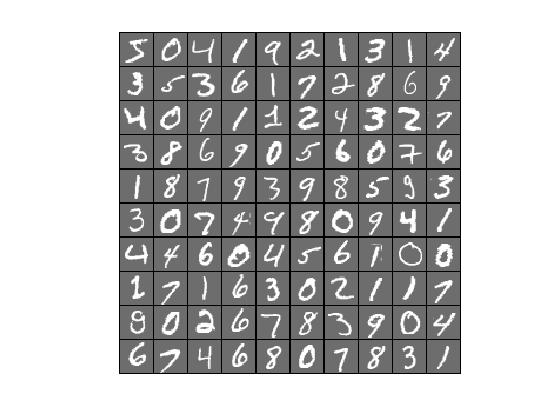
\includegraphics[width=0.8\textwidth]{images/letters.jpg}
\end{figure}

\end{example}

\begin{example}(Linear regression)
Recall from Lecture 1 the problem of finding a function of the form
\begin{equation*}
  Y = \beta_0+\beta_1X_1+\cdots +\beta_pX_p.
\end{equation*}
Given a set of input-output pairs $(\vct{x}_i,y_i)$, arranged in a matrix $\mtx{X}$ and a vector $\vct{y}$, we saw that we could {\em guess} the correct $\vct{\beta} = (\beta_0,\beta_1,\dots, \beta_p)^{\trans}$ by solving the {\em least-squares} optimization problem
\begin{equation*}
  \mathop{\minimize}_{\vct{\beta}} \norm{\mtx{X}\vct{\beta}-\vct{y}}_2^2.
\end{equation*}
By now, we know how to solve this problem using gradient descent.
\end{example}

\begin{example}
In text classification, the task is to decide to which of a given set of categories a given text belongs. The training data consists of a {\em bag of words}: this is a large sparse matrix, whose
columns represent words and the rows represent articles, with the $(i,j)$-th entry containing the number of times word $j$ is contained in text $i$. 

\begin{center}
\begin{tabular}{|r|c|c|}
 & Rooney & Boris \\
\hline 
 Article 1 & 5 & 0 \\
 Article 2 & 1 & 7 \\
\end{tabular}
\end{center}

For example, in the above set we would classify the first article as "Sports" and the second one as "Politics". One such training dataset is the
Reuters Corpus Volume I (RCV1), an archive of over 800,000 categorised newswire stories.

A typical binary classifier for such a problem would be a \textbf{linear classifier} of the form
\begin{equation*}
  h(\vct{x}) = \vct{w}^{\trans}\vct{x}-\tau,
\end{equation*} 
with $\vct{w}\in \R^n$ and $\tau\in \R$. Given a text, represented as a row of the dataset $\vct{x}$, it is classified into one of two classes $\{+1,-1\}$, depending on whether $h(\vct{x})>0$ or $h(\vct{x})<0$. 
\end{example}

Suppose we have the training data $\{\vct{x}_i,y_i\}_{1\leq i\leq m}$ and we found a candidate function $h\colon \mathcal{X}\to \mathcal{Y}$. How do we assess if this is a good fit? One usually assigns to the problem a \textbf{loss function} $\ell\colon \mathcal{Y}\times \mathcal{Y}\to \R_+$ that measures the mismatch of a prediction. One would then aim to find a function $h$ among a set of candidates that minimizes the loss when applying the function to the training data:

\begin{equation*}
  \mathop{\minimize}_{h} \ \frac{1}{m} \sum_{i=1}^m \ell(h(\vct{x}_i,y_i).
\end{equation*}

The form of the loss function depends on the problem at hand, but two typical candidates are the \textbf{square error} for regression problems,
\begin{equation*}
  \ell(h(\vct{x}),y) = (h(\vct{x})-y)^2,
\end{equation*}
and the indicator loss function
\begin{equation*}
  \mathbf{1}\{h(\vct{x})\neq y\},
\end{equation*}
where $\mathbf{1}\{A\}$ is the indication function, which takes the value $1$ if $A$ is true, and $0$ else. As this function is not continuous, in practice one often encounters the {\em log loss} function,
\begin{equation*}
  \ell(h(\vct{x}),y) = \log\left(1+e^{-h(\vct{x})y} \right).
\end{equation*}
Note that if $h(\vct{x})$ and $\vct{y}$ have the same sign (corresponding to a match), then the value of this function will be close to zero. 

Suppose we have a binary classification task at hand, with $\mathcal{Y}=\{-1,1\}$. We could {\em learn} the following function from our data:
\begin{equation*}
  h(\vct{x}) = \begin{cases}
    y_i & \text{ if } \vct{x}=\vct{x}_i,\\
    1 & \text{ otherwise.}
  \end{cases}
\end{equation*}
The \textbf{empirical misclassification risk} in for this problem is then $0$,
\begin{equation*}
  R(h) = \frac{1}{m} \sum_{i=1}^m \mathbf{1}\{h(\vct{x}_i\neq y_i\} = 0.
\end{equation*}
Nevertheless, this is not a good classifier: it will not perform very well outside of the training set. This is an example of \textbf{overfitting}: when the function is adapted too closely to the seen data. To remedy this, one often (randomly) splits the available data into a \textbf{training set} and a \textbf{test set}. The training set is used to find the function $h$, while the test set is for testing how good it is (in practise, one often adds a validation set, used to tune some parameters of the problem).

\begin{example}
In the linear regression problem with the quadratic loss function, we end up with the minimization problem
\begin{equation*}
  \mathop{\minimize}_{\vct{\beta}} \frac{1}{n} \sum_{i=1}^n (\vct{x}_i^{\trans}\vct{\beta}-y_i)^2 =\frac{1}{n}\norm{\mtx{X}\vct{\beta}-\vct{y}}_2^2.
\end{equation*}
This is precisely the problem encountered in Lecture 1.
\end{example}

\begin{example}
In the example of classifying a text into two classes using a linear classifier, we can look at the problem
\begin{equation*}
 \mathop{\minimize}_{\vct{w}, \tau} \frac{1}{n}\sum_{i=1}^m \mathbf{1}\{\vct{w}^{\trans}\vct{x}_i-\tau \neq y_i\}.
\end{equation*}
Since this function is not smooth or even continuous, we can work with the log-loss function described above,
\begin{equation*}
\mathop{\minimize}_{\vct{w}, \tau} \frac{1}{n} \sum_{i=1}^m \ell(\vct{w}^{\trans}\vct{x}_i-\tau, y_i).
\end{equation*}
This function can, in principle, be minimized using gradient descent or Newton's method. 
\end{example}

We have seen how a machine learning problem can be turned into an optimization problem. Unfortunately, when the amount of data is large, computing gradients and Hessians of the resulting functions can be very expensive. Suppose the function $h$ depends on parameters $\vct{w}$ which we want to optimize over, $h=h(\vct{x}; \vct{w})$, and denote the composition of the loss function $\ell$ with $h$ on the data $\vct{x}_i$ by
\begin{equation*}
  f_i(\vct{w}) := \ell(h(\vct{x}_i; \vct{w}),y_i).
\end{equation*}
We can then write our optimization problem as
\begin{equation*}
  \mathop{\minimize}_{\vct{w}} F(\vct{w}), \quad F(\vct{w}) = \frac{1}{m} \sum_{i=1}^m f_i(\vct{w}).
\end{equation*}
The gradient is then
\begin{equation*}
  \nabla F(\vct{w}) = \frac{1}{m} \sum_{i=1}^n \nabla f_i(\vct{w}).
\end{equation*}
For large datasets (for example, $m>10^6$ is not uncommon), computing all the gradients in each step is highly ineffective.

An old algorithm that has recently been revived in light of big data is \textbf{stochastic gradient descent}. The idea is to compute, at each step, only the gradient of {\em one} of the summands of the loss function:

\begin{equation*}
  \vct{w}_{k+1} = \vct{w}_k-\alpha_k \nabla f_{i_k}(\vct{w}_k),
\end{equation*}
where the index $i_k$ is {\em chosen at random} from $\{1,\dots,m\}$ at each step. 

Each step of this algorithm is clearly faster than gradient descent, but does it even work? It turns out that this algorithm converges quickly and that it is surprisingly effective on large datasets.


% %-----------------------------------------------------------------------
% % End of chap1.tex
% %-----------------------------------------------------------------------


%\appendix
%\include{appendix1}

%\backmatter
%\include{biblio}
%\include{index}
\end{document}

%-----------------------------------------------------------------------
% End of chapter.tex
%-----------------------------------------------------------------------
